\subsection{Overview of the article}
The article, "Leadership and Learning at Work: A Systematic Literature Review of Learning-oriented
Leadership", was published on October 25, 2022, in the Journal of Leadership \& Organizational
Studies. It aims to synthesize and evaluate 105 studies on the relationship between leadership and
learning. The paper focuses on exploring leadership approaches that support learning at three
levels: individual, team, and organizational.

The article focuses on three main objectives:

First, it synthesizes existing research related to the connection between leadership and learning,
showing that leaders can promote learning through various styles such as transformational,
supportive, and creative leadership. These styles enhance employees' problem-solving skills and
reflective thinking, thus fostering individual and team learning.

Second, it analyzes and highlights mediating factors, demonstrating that organizational culture,
psychological safety, and team engagement play a critical role in the relationship between
leadership and learning. This underscores that leaders not only directly but also indirectly
influence organizational learning and development through environmental factors.

Third, the article suggests directions for future research, including further exploration of
moderating factors such as industry, gender, and other organizational structures that may impact the
relationship between leadership and learning. Additionally, there is a call for more in-depth
studies on specific leadership behaviors that promote learning, as well as the development of more
accurate measurement tools for learning in the workplace.

\subsection{Methodology}

\subsubsection{Sources of Records}
To locate relevant studies, the primary databases used were Scopus and Web of Science, chosen for
their broad and interdisciplinary scope, making them highly applicable for researching the
leadership-learning relationship. The researchers also searched two additional databases, Emerald
and Business Source, but these did not yield any new studies. The searches in Scopus generated a
total of 8,283 hits, while Web of Science produced 4,178 hits. After removing duplicates, this
resulted in 8,954 unique hits. Beyond the database searches, 23 additional studies were identified
through serendipitous findings—studies not found in the database but encountered during the review
process.

\subsubsection{Reviewing Process}
The team employed a comprehensive search strategy that combined leadership- and learning-related
terms to capture a broad range of studies. Keywords related to leadership included terms like
"leader*", "manage*”, and "supervisor*”. Learning-related terms included "workplace learning”,
"learning at work”, "learning in the workplace”, "work-based learning”, "organizational learning”,
"learning organization”, and "informal learning”. Additionally, specialized terms such as
"learning-oriented leadership”, "learning-centered leadership”, "leadership for learning”, and
"learning leadership” were used. These search terms were developed based on the study's research
questions, existing literature, and collaborative discussions among the team members.

The review process adhered to systematic guidelines (Page et al., 2021) to ensure a thorough and
reliable filtering process. First, an initial screening involved reviewing titles and abstracts
against inclusion criteria, with potentially relevant or hard-to-assess studies moved to a full-text
eligibility assessment. Out of 1,124 studies initially identified, 1,017 full-text articles were
assessed in detail. Ultimately, 136 studies met all inclusion criteria, though some were excluded
due to data duplication, leaving 100 relevant studies. Additionally, 23 studies identified
serendipitously were reviewed, with five meeting quality standards and included in the final
analysis.

\subsubsection{Evaluation Metrics}
The inclusion criteria required that studies focus on (P) working life and workplace contexts, (E)
leadership styles, behaviors, or roles, and (O) employee learning. Eligible studies were
peer-reviewed scientific articles published in international academic journals, written in English,
and containing empirical data collected in workplace settings. These studies needed to statistically
test the relationship between leadership and learning, with a focus on how leaders promote workplace
learning. Exclusion criteria ruled out studies on non-workplace learning (e.g., teacher-student
relationships in education), qualitative studies, and studies that addressed learning outcomes
without exploring the learning process.

To ensure rigor, a quality assessment template \cite{Tompa2007} categorized studies into low,
medium, and high quality, with only medium- and high-quality studies included in the final review.
This assessment narrowed the database-sourced studies to 100, and an additional 5 serendipitous
studies were also included after passing quality checks, resulting in a total of 105 studies.

\begin{figure}
    \centering
    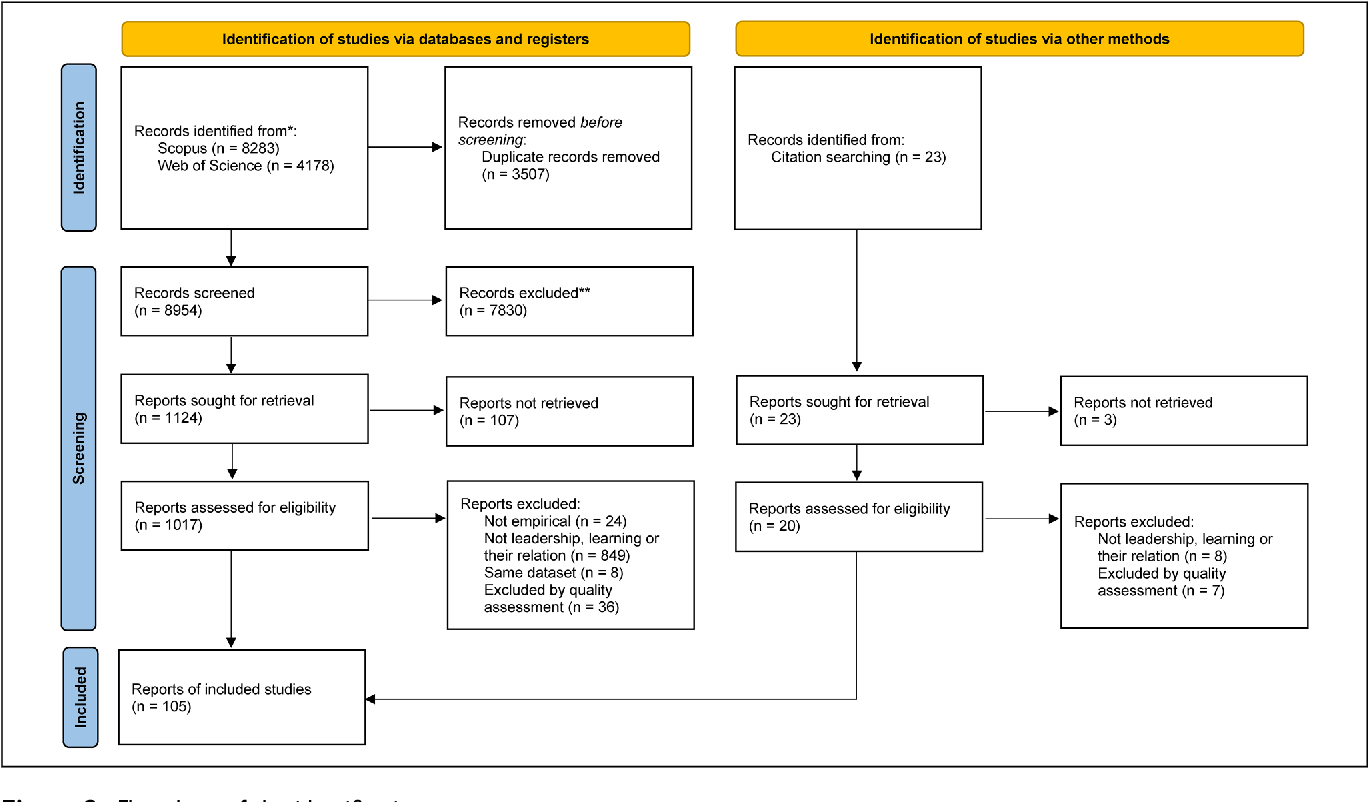
\includegraphics[width=0.9\linewidth]{figures/identification-process.png}
    \caption{Flowchart of the identification process \cite{Lundqvist2022LeadershipAL}}
    \label{fig:identification-process}
\end{figure}

In the final review, 105 studies were analyzed using a narrative synthesis. Central information,
such as leadership constructs and mediators, was compiled and grouped into categories, enabling the
identification of patterns. Leadership theories were classified into five categories based on the
framework by \cite{DINH201436}, while learning was categorized into organizational, group, or
individual learning according to the survey instruments used in each study. This categorization
provided a structured understanding of how various leadership styles influence learning at different
levels within organizations.
